\documentclass[12pt,letterpaper,noanswers]{exam}
\usepackage[usenames,dvipsnames,svgnames,table]{xcolor}
\usepackage[margin=0.9in]{geometry}
\renewcommand{\familydefault}{\sfdefault}
\usepackage{multicol}
\pagestyle{head}
\definecolor{c03}{HTML}{FFDDDD}
\header{AM 108 Class 08}{}{2d Linear Systems}
\runningheadrule
\headrule
\usepackage{graphicx} % more modern
\usepackage{amsmath} 
\usepackage{amssymb} 
\usepackage{hyperref}
\usepackage{tcolorbox}

\begin{document}
 \pdfpageheight 11in 
  \pdfpagewidth 8.5in

\noindent 





\begin{itemize}
\itemsep0em
    \item There is a pre-class assignment for Wednesday.
   % \item Problem Set 02 will be due this Friday.
    \item There is a two question skill check on Wednesday.  The question info is below.
    \item Find office hours info on the Canvas page.
    \item Our first quiz will be on Monday Sept 28th (there is no class meeting that day).  I will post more info tomorrow.
\end{itemize}

\hrule
\vspace{0.2cm}


\noindent\textbf{Teams}

\begin{multicols}{2}
1. 
\end{multicols}

\noindent \textbf{Teams 1 and 2}: Post screenshots of your work to the course Google Drive today.  Include words, labels, and other short notes that might make those solutions useful to you or your classmates.  Find the link in Canvas (or here: \url{https://drive.google.com/drive/u/0/folders/1GcpwvKHD4tMecpFQ4lNxN_r5Ylj7YHbd})


\vspace{0.2cm}
\hrule
\vspace{0.2cm}


\noindent \textbf{Extra vocabulary / extra facts:}
\begin{tcolorbox}
A linear system is \textbf{hyperbolic} if all of its eigenvalues have nonzero real parts.

A linear system is \textbf{non-hyperbolic} otherwise.

A set $M$ is called \textbf{invariant} if orbits that start in $M$ remain in $M$ for all $t\in\mathbb{R}$.

A set $M$ is called \textbf{forward invariant} if orbits that start in $M$ remain in $M$ in forward time.

A \textbf{separatrix} is an invariant curve that separates phase space into regions.  The word is used differently in different texts but it often refers to a separation of the phase space where trajectories in the separated regions have qualitatively different behavior.  The stable manifold of a saddle point is sometimes referred to as a separatrix.


The \textbf{stable subspace}, $E^s$, of a linear system is the span of the eigenvectors whose associated eigenvalues have negative real part.

The \textbf{unstable subspace}, $E^u$, of a linear system is the span of the eigenvectors whose associated eigenvalues have positive real part.

The \textbf{center subspace}, $E^c$, of a linear system is the span of the eigenvectors whose associated eigenvalues have zero real part.

\end{tcolorbox}

\vspace{0.2cm}
\hrule
\vspace{0.2cm}

\noindent\textbf{Addressing your questions}

\begin{enumerate}
\itemsep0em
    \item What are trajectories?  What are straight-line solutions?
    \item How do we find straight-line solutions?
    \item How do eigenvectors and eigenvalues tell us about the shape of trajectories?
    \item When both eigenvalues are negative, what is the intuition for how the trajectories approach the origin?
    \item In 2d linear systems, what kinds of long-term behaviors are possible?  Can solutions approach a vector direction in addition to a fixed point?  (Would they approach a plane in 3d?)
    \item For a degenerate node, where  a solution $\underline{x}(t)$ is given by $\underline x(t) = c_1 \underline{v}e^{\lambda t} + c_2(\underline{v} t + \underline{u})e^{\lambda t}$, how does this result in the phase portrait that we see?
    \item When we define Liapunov stability, what do we mean by 'close' to $x^*$, and what is a large excursion (vs staying close)?
    \item Why are the fixed points in a line of fixed points considered Liapunov stable?
    \item When will there be fixed points away from the origin in a 2d system?
\end{enumerate}

\vspace{0.2cm}

\hrule
\vspace{0.2cm}

\noindent\textbf{Skill Check C09 practice}
\begin{questions}

\item Identify nondimensional groups in a differential equation (see the C06 skill check or the C05 handout for an example).

\item Consider the 2d linear system $\dot x = 3x+y$, $\dot y = x-y$.  This system can also be written $\displaystyle \frac{d}{dt}\left(\begin{array}{c} x \\ y \end{array}\right) = \left(\begin{array}{c c} 3 & 1 \\ 1  & -1 \end{array}\right)\left(\begin{array}{c} x \\ y \end{array}\right)$.

\[\left(\begin{array}{c} x(t) \\ y(t) \end{array}\right) = 2e^{(1+\sqrt{5})t}\left(\begin{array}{c} 2+\sqrt{5} \\ 1 \end{array}\right)+3e^{(1-\sqrt{5})t}\left(\begin{array}{c} 2-\sqrt{5} \\ 1 \end{array}\right)\] is a solution to this system.

Match this system to its corresponding phase portrait below.

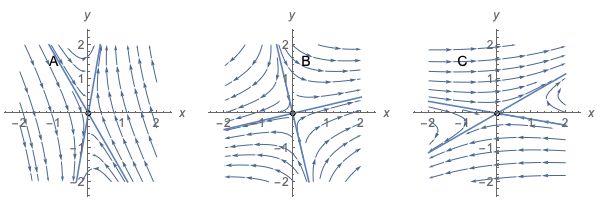
\includegraphics[width=\linewidth]{img/C08prac-2019-09-20.png}

\bgroup
\def\arraystretch{2}
\begin{tabular}{|c|p{2cm}|}
\hline
Match:    &  \\
     \hline
\end{tabular}
\egroup
\end{questions}

\vspace{0.2cm}

\hrule
\vspace{0.2cm}

\noindent\textbf{Skill Check C09 practice solution}

2. The solution we were given is the weighted sum of an exponentially growing component, and an exponentially decaying one.  Presumably $(2+\sqrt{5},1)^T$ and $(2-\sqrt{5}, 1)^T$ are the eigenvectors of the system.  I'll check that:

$\left(\begin{array}{c c} 3 & 1 \\ 1  & -1 \end{array}\right)\left(\begin{array}{c} 2\pm\sqrt{5} \\ 1 \end{array}\right) = \left(\begin{array}{c} 6 \pm 3\sqrt{5} + 1 \\ 2\pm \sqrt{5} - 1\end{array}\right) = \left(\begin{array}{c} 7 \pm 3\sqrt{5} \\ 1\pm \sqrt{5} \end{array}\right) = (1\pm\sqrt{5})\left(\begin{array}{c} 2\pm\sqrt{5} \\ 1 \end{array}\right)$.

We have an exponentially growing solution $(1+\sqrt{5})\left(\begin{array}{c}2 + \sqrt{5} \\ 1\end{array}\right)$.  This will be a straight line along which trajectories move outward.  For every four units in $x$, we go up one in $y$ along this line.  Based on this, I can eliminate A from the options.

We have an exponentially decaying solution $(1-\sqrt{5})\left(\begin{array}{c}2 - \sqrt{5} \\ 1\end{array}\right)$.  This will be a straight line along which trajectories move towards the origin.  $2 - \sqrt{5}$ is negative but close to zero.  So we move a small distance along the negative $x$ axis for each unit upwards in $y$.  That means the match is B.

\vspace{0.2cm}

\hrule
\vspace{0.2cm}

\eject

\begin{questions}
\item (1d vs 2d)
\begin{parts}
    \item Consider the dynamical system $\dot{x} = f(x)$ with $f(x) = x - x^2$.  I haven't always managed to carefully distinguish between a \emph{vector field} and a \emph{phase portrait} because they look very similar in 1d.
    
    Here is a plot of the vector field.  The vector field is an assignment of the vector $f(x)\vec i$ to the point $x$. 
    
    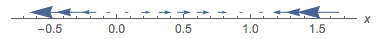
\includegraphics{img/S19-C071dvector.png}
    
    \begin{itemize}
        \item Sketch the phase portrait (drawn on the phase line) for this system on the axis below.
        
        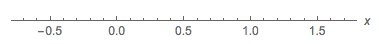
\includegraphics{img/S19-C07-1daxis.png}
        \item Identify how the phase portrait is similar to or different from the vector field.
        \item How do trajectories appear in the 1d phase portrait?
    \end{itemize}
\item Now consider the dynamical system $\begin{array}{c} \dot{x} = f(x,y) \\ \dot{y} = g(x,y)\end{array}$.  The vector field is an assignment of the vector $f(x,y)\vec i + g(x,y)\vec j$ to the point $(x,y)$.  Let $f(x,y) = x-2y, g(x,y) = 3x+y.$

Consider the two images below.  Which one is the vector field (plotted in the phase plane), and which one is the phase portrait (drawn on the phase plane)?

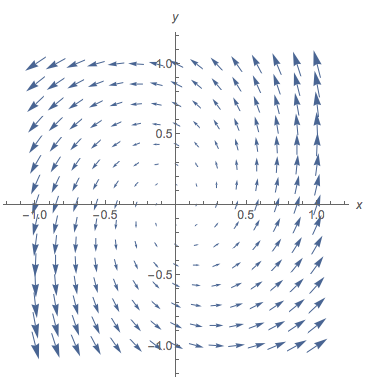
\includegraphics[width=0.5\linewidth]{img/S19-C07-2dvector.png}
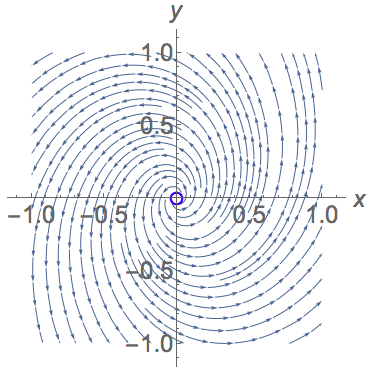
\includegraphics[width=0.5\linewidth]{img/S19-C07-2dphase.png}

Identify how the phase portrait is similar to or different from the vector field.
\end{parts}

\textbf{Answers}:

A vector field places a vector at each point on a line or in a plane.  We interpret that vector as providing the speed (and direction) of our particle, so the vector field displays speed and direction information.
The phase portrait shows trajectories, the direction of time, and fixed points, but no information about speed.

\item (Generic 2d system of linear differential equations) 

Consider the system 
\begin{align*}
\frac{dx}{dt} =&\ ax + by \\
\frac{dy}{dt} =&\ cx + dy
\end{align*}
with fixed point at the origin.
\begin{parts}
\item Rewrite this in matrix / vector form (let $\displaystyle \underline{x} = \left(\begin{array}{c} x \\ y \end{array}\right).)$
\item Let $\displaystyle A = \left(\begin{array}{c c} a & b \\ c & d \end{array}\right).$  Recall that the eigenvalues of $A$, $\lambda_1$ and $\lambda_2$, are given by $\lambda^2 - \tau \lambda + \Delta = 0$ where $\tau = a +d $ is the trace of the matrix $A$ and $\Delta = ad - bc$ is the determinant of the matrix $A$.  In addition, $(\lambda - \lambda_1)(\lambda-\lambda_2) = 0$.  Why?
\item Use this second fact (and match terms in the two equations) to show that $\lambda_1 + \lambda_2 = \tau$ and $\lambda_1\lambda_2 = \Delta$.
\item Consider the $\Delta\tau$-plane (with $\Delta$ on the horizontal axis).  Identify regions of the $\Delta\tau$ plane where the matrix has two negative eigenvalues, regions where it has one positive eigenvalue and one negative one, and regions where it has two positive eigenvalues.
\item Consider $\underline{v}e^{\lambda_1 t}$, where $\lambda_1$ is an eigenvalue of $A$ and $\underline{v}$ is the associated eigenvector.  Show that this is a solution of the differential equation (Steve did this in the linear systems video, and it's fine to follow his steps).  Think about plotting this solution as a trajectory in the $xy$-plane.  Why is it a straight-line solution?
\item General solutions to this differential equation are of the form $\displaystyle\underline{x}(t) = c_1\underline{v}_1e^{\lambda_1 t} + c_2\underline{v}_2e^{\lambda_2 t}$.  We might have $\lambda_1$ and $\lambda_2$ both real.  Or they could be a complex conjugate pair, where $\lambda_1 = \lambda+i\omega$ and $\lambda_2 = \lambda-i\omega$.  When they are a complex conjugate pair, we require the solution to the differential equation to be real, so we require $c_1$ and $c_2$ to be a complex conjugate pair as well.

For the systems
\[ 
\begin{array}{ r l c r l c r l c r l c}
 \dot{x} =  &x  & \quad & \dot{x} = &-x - y & \quad & \dot{x} = &\ x & \quad & \dot{x} =&\ x + y \\
 \dot{y} = &x- y & \quad & \dot{y} = &\ x - 2y & \quad & \dot{y} = &- y & & \dot{y} = &-2x + y\\
\end{array}\]
find their trace and their determinant.  Which have real eigenvalues and which have eigenvalues that are a complex conjugate pair?

\item Attempt to match the systems above to the phase portraits below.

\includegraphics[width=5in]{img/VectorFields.pdf}

%For what conditions on $\lambda_1$ and $\lambda_2$ (and thus on $\tau$ and $\Delta$) would all solutions eventually approach the fixed point at $\underline{x} = \underline{0}$?
\end{parts}
\eject 
\textbf{Answers:}
2a: $\displaystyle \underline{x} = \left(\begin{array}{c} x \\ y \end{array}\right)$, $\displaystyle \dot{\underline{x}} = \frac{d}{dt}\left(\begin{array}{c} x \\ y \end{array}\right),$ $A = \left(\begin{array}{c c} a & b \\ c & d \end{array}\right)$.  The equation becomes $\dot{\underline{x}} = A\underline{x}$.

2b: $(\lambda - \lambda_1)(\lambda - \lambda_2) = 0$ because the eigenvalues $\lambda_1$ and $\lambda_2$ are the roots of the characteristic equation.

2c: Expanding, $\lambda^2 - (\lambda_1+\lambda_2)\lambda + \lambda_1\lambda_2 = 0$.  We have $\lambda^2 - \tau \lambda + \Delta$ and $\lambda^2 - (\lambda_1+\lambda_2)\lambda + \lambda_1\lambda_2$.  These polynomials have the same roots and the same leading coefficient: they are the same polynomial.  So $\tau = \lambda_1+\lambda_2$ and $\Delta = \lambda_1\lambda_2$.


2d: The left side has $\Delta<0$ so one positive and one negative.  The first quadrant has two positive eigenvalues.  The fourth quadrant has two negative.

2e: $\underline{x} = \underline{v}e^{\lambda_1 t}$.  $\dot{x} = \underline{v} \lambda_1 e^{\lambda_1 t}$.  $A\underline{x} = A\underline{v}e^{\lambda_1 t}$.  $\underline{v}$ is an eigenvector of $A$ so $A\underline{v} = \lambda_1 \underline{v}$.  The sides match.  This is a straight line solution because the solution is a constant multiple of a single vector direction, so we move along that direction (either exponential growth, or exponential decay) as time increases.

2f: 

\begin{tabular}{c | c | p{3cm} | p{6cm}}
    $\left(\begin{array}{c c} 1 & 0 \\ 1 & -1 \end{array}\right)$ & $\tau = 1+-1 = 0$& $\Delta = 1(-1) - (0)(1) = -1$ & $\Delta < 0$. real eigenvalues\\
    $\left(\begin{array}{c c} -1 & -1 &  \\ 1 & -2 \end{array}\right)$ & $\tau = -1 + -2 = -3$ & $\Delta = -1(-2) - (-1)(1) = 3$ & $\lambda_{\pm} = \tau/2 \pm \frac{1}{2}\sqrt{\tau^2-4\Delta}.$  $\tau^2-4\Delta = 9-12 = -3$ so complex\\
    $\left(\begin{array}{c c} 1 & 0 \\ 0 & -1 \end{array}\right)$ & $\tau = 1 + -1 = 0$ & $\Delta = 1(-1) - (0)(0) = -1$ & $\Delta < 0$. real eigenvalues\\
    $\left(\begin{array}{c c} 1 & 1 \\ -2 & 1 \end{array}\right)$ & $\tau = 1 + 1 = 2$ & $\Delta = 1(1) - (1)(-2) = 3$ & $\lambda_{\pm} = \tau/2 \pm \frac{1}{2}\sqrt{\tau^2-4\Delta}.$  $\tau^2-4\Delta =4-12 = -8$ so complex
\end{tabular}

2g: 
$\begin{array}{r l c} \dot{x} = &\ x  \\ \dot{y} = &- y\end{array} $ has eigenvectors along the axes so matches to the upper left plot.

$\begin{array}{r l c} \dot{x} = &\ x  \\ \dot{y} = &x- y\end{array} $ is the other saddle point so matches to the upper right plot.

Not sure how to match the two spirals.  One has a larger complex component than the other, so I might guess that one matches with the more swirly plot (bottom left).


% \eject

% \item (Solutions to second order linear constant-coefficient equations) \\
% We couldn't deal with second order ODEs with the methods of the first part of the course.  All of our reasoning required us to be working with a first order ODE.  We'll be able to work with this kind of equation now, though.  Consider the equation
% \[\ddot{x} + \dot{x} - 2 x = 0. \]
% \begin{parts}
% \item 
% Consider a possible solution to the differential equation, $x(t) = A e^{rt}$.  Using the method of substitution (i.e. sub this ansatz in to the equation), determine $r$ so that this is a solution.
% \item You should have found two possible values of $r$.  Do those values correspond to solutions showing 
% exponential growth or exponential decay?   \emph{This should remind you of the process for finding eigenvalues.  }
% \item We still can't work directly with second order ODEs.  However, we can translate them into a system of two first order ODEs.  In order to do that, we think of $y = \dot{x}$ as a second variable, so $x, y$ are the two variables in our system.  The ODE is now a system of two equations, 
% \[\dot{x} = y, \quad \dot{y} + y - 2x = 0.\]  Find the matrix $A$ associated with this system, and find its eigenvalues.  How do they relate to the values of $r$ you found above?

% Mathematica syntax:
% \begin{verbatim}
% Eigenvalues[{{a, b}, {c, d}}]
% \end{verbatim}
% \item Consider the third order equation $\dddot{x}+\ddot{x}+x^2 = 0$.  Let $y = \dot{x}, z = \dot{y}$.  Use this to rewrite the equation as a first order system of the form
% \begin{align*}
%  \dot{x} = &\ y \\
%  \dot{y} = &\ z \\
%  \dot{z} = &
% \end{align*}

%\item
%The general solution of the differential equation is written as an arbitrary linear combination of $e^{r_1 t}$ and $e^{r_2 t}$.
%Write down the general solution.
%\item Find $\dot{x}(t)$, the derivative with respect to time of the general solution (this will be useful in the next question).
%\end{parts}

%\item Use trace and determinant to match the following systems to one of the phase portraits below.  
%If necessary, use eigenvectors as well.
%
%\[ 
%\begin{array}{ r l c r l c r l c r l c}
% \dot{x} =  &x  & \quad & \dot{x} = &-x - y & \quad & \dot{x} = &\ x & \quad & \dot{x} =&\ x + y \\
% \dot{y} = &x- y & \quad & \dot{y} = &\ x - 2y & \quad & \dot{y} = &- y & & \dot{y} = &-2x + y\\
%\end{array}\]
%
%\includegraphics[width=5in]{VectorFields.pdf}

%\item ({\color{blue} extra, if you like probability} 5.3.14) Suppose we pick a linear system at random.  What's the probability the origin will be stable, unstable, or a saddle?  \\  To be more specific about what we mean by ``random'', consider the system $\dot{\underline{x}} = A\underline{x}$, where $A=\left(\begin{array}{c c} a & b \\ c & d \end{array}\right)$.  Suppose we pick the entries $a,b,c,d$ independently and at random from a uniform distribution on the interval $[-1,1]$.

\end{questions}

\end{document}